\clearpage

\section{Transparent with 1+1 Protection}
In this case study we focus on the transparent case with 1 + 1 protection.
In this mode of transport, the information travels in a route defined through optical channels between origin and destination nodes always in the optical domain and, consequently, physical topology and logical topology are different.
An advantage of this mode of transport is the possibility of transporting express traffic.
An disadvantage is that the capacity utilization of the optical channels is worse than in the opaque mode of transport due to grooming only customer signs with the same endpoints.

\subsection{Physical Network Topology}
\begin{tcolorbox}	
\begin{tabular}{p{2.75cm} p{0.2cm} p{10.5cm}} 	
\textbf{Student Name}  &:& Tiago Esteves    (October 03, 2017 - )\\
\textbf{Goal}          &:& Implement the dimensioning of optical networks in the transparent transport mode.
\end{tabular}
\end{tcolorbox}
\vspace{-5pt}

\subsubsection{Reference Network}
In the figure below we ca see that our reference network consists of 6 nodes and 8 Bidirectional links.
The matrix of distances between the respective nodes and the ODU's matrices are the same as those reported in the opaque transport mode.

\begin{figure}[h!]
\centering
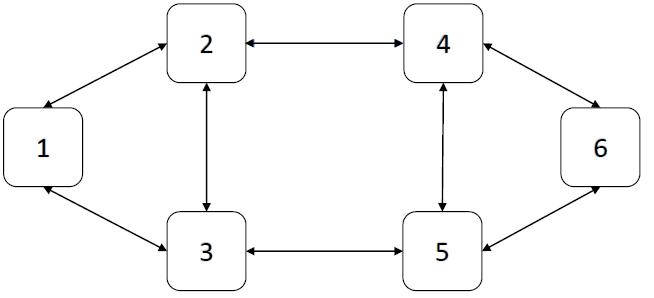
\includegraphics[width=\textwidth]{RedeTeste}
\caption{Physical Topology of the Reference Network.}
\end{figure}

The distance matrix is the same for the two scenarios but the ODU's matrices are not.
In this case only the matrices for the case of high traffic are elucidated, being that in the case of a low traffic it is only necessary to divide these matrices by the value 10.

\[
Dist=
  \begin{bmatrix}
    0 & 500 & 500 & 0 & 0 & 0 \\
    500 & 0 & 400 & 500 & 0 & 0 \\
    500 & 400 & 0 & 0 & 500 & 0 \\
    0 & 500 & 0 & 0 & 600 & 450 \\
    0 & 0 & 500 & 600 & 0 & 550 \\
    0 & 0 & 0 & 450 & 550 & 0
  \end{bmatrix}
\quad ODU0=
  \begin{bmatrix}
    0 & 50 & 10 & 30 & 10 & 30 \\
    50 & 0 & 0 & 10 & 50 & 0 \\
    10 & 0 & 0 & 10 & 40 & 10 \\
    30 & 10 & 10 & 0 & 10 & 0 \\
    10 & 50 & 40 & 10 & 0 & 30 \\
    30 & 0 & 10 & 10 & 30 & 0
  \end{bmatrix}
\]
\[
ODU1=
  \begin{bmatrix}
    0 & 20 & 40 & 20 & 0 & 50 \\
    20 & 0 & 0 & 30 & 10 & 10 \\
    40 & 0 & 0 & 10 & 10 & 0 \\
    30 & 30 & 10 & 0 & 10 & 30 \\
    0 & 10 & 10 & 10 & 0 & 10 \\
    50 & 10 & 0 & 30 & 10 & 0
  \end{bmatrix}
\quad ODU2=
  \begin{bmatrix}
    0 & 10 & 10 & 10 & 0 & 0 \\
    10 & 0 & 0 & 0 & 10 & 0 \\
    10 & 0 & 0 & 10 & 10 & 0 \\
    10 & 0 & 10 & 0 & 10 & 0 \\
    0 & 10 & 10 & 10 & 0 & 10 \\
    0 & 0 & 0 & 0 & 10 & 0
  \end{bmatrix}
\]
\[
ODU3=
  \begin{bmatrix}
    0 & 0 & 0 & 0 & 0 & 0 \\
    0 & 0 & 10 & 0 & 0 & 10 \\
    0 & 10 & 0 & 0 & 10 & 0 \\
    0 & 0 & 0 & 0 & 0 & 0 \\
    0 & 0 & 10 & 0 & 0 & 0 \\
    0 & 10 & 0 & 0 & 0 & 0
  \end{bmatrix}
\qquad ODU4=
  \begin{bmatrix}
    0 & 0 & 0 & 0 & 0 & 0 \\
    0 & 0 & 0 & 0 & 0 & 10 \\
    0 & 0 & 0 & 0 & 0 & 0 \\
    0 & 0 & 0 & 0 & 0 & 0 \\
    0 & 0 & 0 & 0 & 0 & 10 \\
    0 & 10 & 0 & 0 & 10 & 0
  \end{bmatrix}
\]

Through these ODU's we can calculate total network traffic for the low traffic scenario:\\
$T_1^0$ = 600x1.25 = 750 Gbits/s \qquad
$T_1^1$ = 500x2.5 = 1250 Gbits/s \qquad
$T_1^2$ = 160x10 = 1600 Gbits/s \\
$T_1^3$ = 60x40 = 2400 Gbits/s \quad
$T_1^4$ = 40x100 = 4000 Gbits/s \\
$T_{1total}$ = 750 + 1250 + 1600 + 2400 + 4000 = 10000 Gbits/s \qquad
$T_{total}$ = 10000/2 = 5 Tbits/s\\

We can thus conclude that the total traffic for the two scenarios is as follows:
\begin{itemize}
  \item Low Traffic: \textbf{0.5 TBits/s}
  \item High Traffic: \textbf{5 TBits/s}
\end{itemize}

Finally for this project has to take into consideration the table \ref{table:3} because in it we can see the values of the variables associated with this network.
\begin{table}[h!]
\centering
\begin{tabular}{|| c | c | c||}
 \hline
 Constant & Description & Value \\
 \hline\hline
 N & Number of nodes & 6 \\
 L & Number of bidirectional links & 8 \\
 <$\delta$> & Node out-degree & 2.667 \\
 <len> & Mean link length (km) & 500 \\
 <h> & Mean number of hops for working paths & 1.533 \\
 <h'> & Mean number of hops for backup paths & 2.467 \\
 \hline
\end{tabular}
\caption{Table of reference network values}
\label{table:3}
\end{table}


\subsubsection{Realistic Network}
The real network chosen for this work is the EON (European Optical Network).
The way the nodes are arranged geographically can be seen from the following figure and the matrix of distances created in the next page is constructed based on real distances.
In this case just ODU's matrices are created to be able to determine the total traffic used in each scenario.

\begin{figure}[h!]
\centering
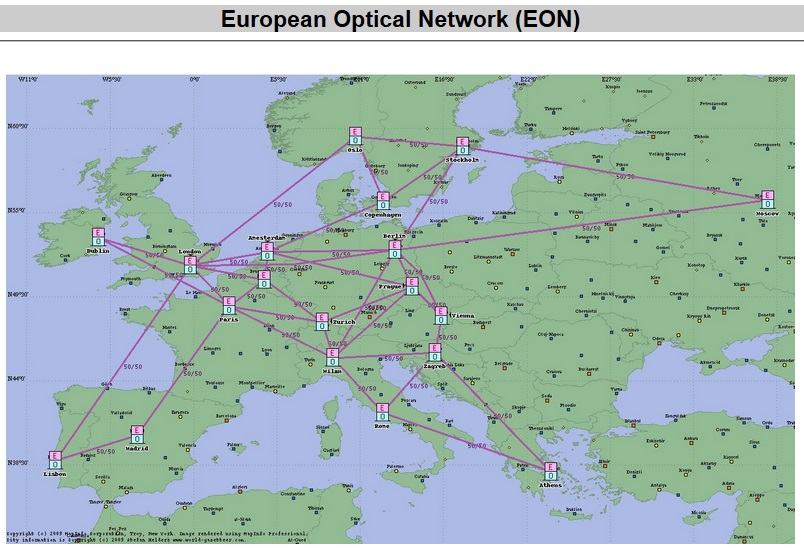
\includegraphics[width=\textwidth]{EON_Rede_Realista}
\caption{Physical Topology of the Realistic Network.}
\end{figure}

The table \ref{table:4} shows the values of the variables associated with this network.
\begin{table}[h!]
\centering
\begin{tabular}{|| c | c | c||}
 \hline
 Constant & Description & Value \\
 \hline\hline
 N & Number of nodes & 19 \\
 L & Number of bidirectional links & 37 \\
 <$\delta$> & Node out-degree & 3.89 \\
 <len> & Mean link length (km) & 753.76 \\
 <h> & Mean number of hops for working paths & 2.3 \\
 <h'> & Mean number of hops for backup paths & 3.2 \\
 \hline
\end{tabular}
\caption{Table of realistic network values}
\label{table:4}
\end{table}

Again, through the ODU's we can calculate the total traffic for both scenarios being them:
\begin{itemize}
  \item Low Traffic: \textbf{2 TBits/s}
  \item High Traffic: \textbf{20 TBits/s}
\end{itemize}


\[
  \text{Dist} = \kbordermatrix{
    & Oslo & Stockholm & Moscow & Copenhagen & Berlin & Prague & Vienna & Zagreb & Athens & Rome & Milan & Zurich & Brussels & Amesterdan & London & Dublin & Paris & Madrid & Lisbon \\
    Oslo & 0 & 500 & 500 & 0 & 0 & 0 & 0 & 500 & 500 & 0 & 0 & 500 & 500 & 0 & 0 & 0 & 0 & 500 & 500 \\
    Stockholm & 0 & 500 & 500 & 0 & 0 & 0 & 0 & 500 & 500 & 0 & 0 & 500 & 500 & 0 & 0 & 0 & 0 & 500 & 500 \\
    Moscow & 0 & 500 & 500 & 0 & 0 & 0 & 0 & 500 & 500 & 0 & 0 & 500 & 500 & 0 & 0 & 0 & 0 & 500 & 500 \\
    Copenhagen & 0 & 500 & 500 & 0 & 0 & 0 & 0 & 500 & 500 & 0 & 0 & 500 & 500 & 0 & 0 & 0 & 0 & 500 & 500 \\
    Berlin & 0 & 500 & 500 & 0 & 0 & 0 & 0 & 500 & 500 & 0 & 0 & 500 & 500 & 0 & 0 & 0 & 0 & 500 & 500 \\
    Prague & 0 & 500 & 500 & 0 & 0 & 0 & 0 & 500 & 500 & 0 & 0 & 500 & 500 & 0 & 0 & 0 & 0 & 500 & 500 \\
    Vienna & 0 & 500 & 500 & 0 & 0 & 0 & 0 & 500 & 500 & 0 & 0 & 500 & 500 & 0 & 0 & 0 & 0 & 500 & 500 \\
    Zagreb & 0 & 500 & 500 & 0 & 0 & 0 & 0 & 500 & 500 & 0 & 0 & 500 & 500 & 0 & 0 & 0 & 0 & 500 & 500 \\
    Athens & 0 & 500 & 500 & 0 & 0 & 0 & 0 & 500 & 500 & 0 & 0 & 500 & 500 & 0 & 0 & 0 & 0 & 500 & 500 \\
    Rome & 0 & 500 & 500 & 0 & 0 & 0 & 0 & 500 & 500 & 0 & 0 & 500 & 500 & 0 & 0 & 0 & 0 & 500 & 500 \\
    Milan & 0 & 500 & 500 & 0 & 0 & 0 & 0 & 500 & 500 & 0 & 0 & 500 & 500 & 0 & 0 & 0 & 0 & 500 & 500 \\
    Zurich & 0 & 500 & 500 & 0 & 0 & 0 & 0 & 500 & 500 & 0 & 0 & 500 & 500 & 0 & 0 & 0 & 0 & 500 & 500 \\
    Brussels & 0 & 500 & 500 & 0 & 0 & 0 & 0 & 500 & 500 & 0 & 0 & 500 & 500 & 0 & 0 & 0 & 0 & 500 & 500 \\
    Amesterdan & 0 & 500 & 500 & 0 & 0 & 0 & 0 & 500 & 500 & 0 & 0 & 500 & 500 & 0 & 0 & 0 & 0 & 500 & 500 \\
    London & 0 & 500 & 500 & 0 & 0 & 0 & 0 & 500 & 500 & 0 & 0 & 500 & 500 & 0 & 0 & 0 & 0 & 500 & 500 \\
    Dublin & 0 & 500 & 500 & 0 & 0 & 0 & 0 & 500 & 500 & 0 & 0 & 500 & 500 & 0 & 0 & 0 & 0 & 500 & 500 \\
    Paris & 0 & 500 & 500 & 0 & 0 & 0 & 0 & 500 & 500 & 0 & 0 & 500 & 500 & 0 & 0 & 0 & 0 & 500 & 500\\
    Madrid & 0 & 500 & 500 & 0 & 0 & 0 & 0 & 500 & 500 & 0 & 0 & 500 & 500 & 0 & 0 & 0 & 0 & 500 & 500 \\
    Lisbon & 0 & 500 & 500 & 0 & 0 & 0 & 0 & 500 & 500 & 0 & 0 & 500 & 500 & 0 & 0 & 0 & 0 & 500 & 444
  }
\]


\newpage
\subsection{Dimensioning using ILP}
\begin{tcolorbox}	
\begin{tabular}{p{2.75cm} p{0.2cm} p{10.5cm}} 	
\textbf{Student Name}  &:& Tiago Esteves    (October 03, 2017 - )\\
\textbf{Goal}          &:& Implement the dimensioning of optical networks in the transparent transport mode.
\end{tabular}
\end{tcolorbox}

\subsubsection{ILP Models} \label{ILP_models_Transp}

Again, for a better understanding of the functions and variables used in the ILP, a table \ref{description_transp} will be created with all the variables and their description. \\

\begin{table}[h!]
\centering
\begin{tabular}{ |p{1cm}||p{13cm}|}
 \hline
 \multicolumn{2}{|c|}{Description of notation used in the objective function} \\
 \hline
 \hline
 $i$ & index for start node of a physical link \\
 $j$ & index for end node of a physical link \\
 $o$ & index for node that is origin of a demand \\
 $d$ & index for node that is destination of a demand \\
 $($ i,j $)$ & physical link between the nodes $i$ and $j$ \\
 $($ o,d $)$ & demand between the nodes $o$ and $d$ \\
 $f_{ij}^{od}$ & Number of 100 Gbit/s optical channels (number of flows) between the link $i$ and $j$ for all demand pairs between $o$ and $d$ \\
 $W_{od}$ & number of optical channels between the nodes $o$ and $d$\\
 G & Network topology in form of adjacency matrix \\
 \hline
\end{tabular}
\caption{Table with description of variables}
\label{description_transp}
\end{table}


The optimization model suggested for transparent transport mode with dedicated path protection intends to minimize the total number of flows crossing link (i, j) for all demand pairs (o, d). The mathematical model described below also minimizes the total number of optical channels between each demand end nodes $W_{od}$, instead of minimizing the number of optical link-by-link channels as in the previous model.

\vspace{10pt}
\begin{equation}
minimize    \sum_{(i,j)} \sum_{(o,d)} f_{ij}^{od} + \sum_{(o,d)} W_{od}
\label{ILPTransp}
\end{equation}

$subject$ $to$
\begin{equation}
\sum_{j\textbackslash \{o\}} f_{ij}^{od} = 2  \qquad \qquad \qquad \qquad \qquad \qquad \qquad \qquad \qquad \qquad
\forall(o,d) : o < d, \forall i: i = o
\label{ILPTransp1}
\end{equation}

\begin{equation}
\sum_{j\textbackslash \{o\}} f_{ij}^{od} = \sum_{j\textbackslash \{d\}} f_{ji}^{od}   \qquad \qquad \qquad \qquad \qquad \qquad \qquad \qquad
\forall(o,d) : o < d, \forall i: i \neq o,d
\label{ILPTransp2}
\end{equation}

\begin{equation}
\sum_{j\textbackslash \{d\}} f_{ji}^{od} = 2  \qquad \qquad \qquad \qquad \qquad \qquad \qquad \qquad \qquad \qquad
\forall(o,d) : o < d, \forall i: i = d
\label{ILPTransp3}
\end{equation}

\begin{equation}
\sum_{(o,d):o<d} \left(f_{ij}^{od} + f_{ji}^{od}\right) W_{od} \leq 80 G_{ij} \qquad \qquad \qquad \qquad \qquad \qquad \qquad \qquad
\forall(i,j) : i < j
\label{ILPTransp4}
\end{equation}

\begin{equation}
f_{ij}^{od} , f_{ji}^{od} \in \{0,2\}   \qquad \qquad \qquad \qquad \qquad \qquad \qquad \qquad \qquad
\forall(i,j) : i < j, \forall(o,d) : o < d
\label{ILPTransp5}
\end{equation}

\begin{equation}
W_{od} \in \mathbb{N}  \qquad \qquad \qquad \qquad \qquad \qquad \qquad \qquad \qquad \qquad \qquad \qquad \qquad
\forall(o,d) : o < d
\label{ILPTransp6}
\end{equation}


The objective function, to be minimized, is the expression \ref{ILPTransp}. The flow conservation is performed by equations \ref{ILPTransp1}, \ref{ILPTransp2} and \ref{ILPTransp3} and share the same mathematical description of opaque model. The inequality \ref{ILPTransp4} answers capacity constraint problem. Then, total flows times the traffic of the demands must be less or equal to the capacity of network links. The grooming of this model can be done before routing since the traffic is aggregated just for demands between the same nodes, thus not depending on the routes. Last two constraints define the total number of flows must be zero if there is no demand, or two for a demand with traffic protection, and the number of optical channels must be a counting number.

\subsubsection{ILP Results}

In this initial phase the results will be presented using ILP to calculate the CAPEX of the reference network and the realistic network.
The value of the CAPEX of the network will be calculated based on the costs of the equipment present in the table below.

\begin{table}[h!]
\centering
\begin{tabular}{|| c | c||}
 \hline
 Equipment & Cost \\
 \hline\hline
 OLT without transponders & 15000 \euro \\
 Transponder & 5000 \euro/Gb \\
 Optical Amplifier & 4000 \euro \\
 EXC & 10000 \euro \\
 OXC & 20000 \euro \\
 EXC Port & 1000 \euro /Gb/s\\
 OXC Port & 2500 \euro /porto \\
 \hline
\end{tabular}
\caption{Table with costs}
\label{table_cost2}
\end{table}

In addition to the equipment costs we will also use the parameter "span", which in this case will have a value of 100, because this value is used to calculate the number of optical amplifiers required in the network using Equation \ref{amplifiersTransp}.

\begin{equation}
N^R = \sum\limits_{l=1}^L\left(\left\lceil\frac{len_l}{span}\right\rceil-1\right)
\label{amplifiersTransp}
\end{equation} \\

To know the value of CAPEX it is necessary to know the value of the cost of the links and the cost of the nodes.

To calculate the cost of the nodes, the sum of the costs of the optical and electrical node is made. For this case the optical cost is given by equation \ref{opticalCost} and the electrical cost by the equation \ref{electricalCostTransp}.


\begin{equation}
C_{oxc} = \left(\gamma_{o0} \times N \right) + \gamma_{o1} \times  \left(P_{LINE} + P_{ADD}\right)
\label{opticalCost}
\end{equation}	
	
\begin{itemize}
\item{$C_{oxc}$		$\rightarrow$	Optical Ports Cost}
\item{$\gamma_{o0}$	$\rightarrow$	OXC cost in Euros}
\item{$\gamma_{o1}$	$\rightarrow$	OXC port cost in Euros}
\item{$P_{TRIB}	$	$\rightarrow$	Number of tributary ports}
\item{$P_{ADD} $	$\rightarrow$	Number of adding ports}
\end{itemize}

\begin{equation}
C_{exc} = \left(\gamma_{e0}\times N\right) + \gamma_{e1} \times \left(2 \times T_1 \right)		\label{electricalCostTransp}
\end{equation}

\vspace{10pt}

To calculate the cost of the Links we will use the equation \ref{linkCostsTransp}.

\begin{equation}
C_L = \left(2 \times \gamma_0^{OLT} \times L\right) + \left(2 \times \gamma_1^{OLT} \times \tau \times W\right) + \left(N^R \times c^R\right)
\label{linkCostsTransp}
\end{equation} \\
	
\vspace{11pt}
To perform the calculations using the implementation of the models described in section \ref{ILP_models_OP} it is necessary to use a mathematical software tool. For this we will use MATLAB which is ideal for dealing with linear programming problems and can call the LPsolve through an external interface. \\

\textbf{Scenario 1: Test Network Low Traffic} \label{Scenario1_transp} \\
In this scenario we used the table \ref{table:3}. In the table \ref{result_ILP1_T} we can see the values calculated through MatLab and using the values indicated in table \ref{table_cost2} we can finally calculate the CAPEX value. \\
\newpage
\begin{table}[h!]
\centering
\begin{tabular}{|| c | c || c | c || c | c ||}
 \hline
 Number of optical channels & Value & ADD PORTS & Value & LINE PORTS & Value \\
 \hline\hline
 in the link (1,2) & 3 & Node 1 & 5 & Node 1 & 5 \\
 in the link (1,3) & 2 & Node 2 & 6 & Node 2 & 12 \\
 in the link (2,3) & 4 & Node 3 & 5 & Node 3 & 11 \\
 in the link (2,4) & 5 & Node 4 & 5 & Node 4 & 11 \\
 in the link (3,5) & 5 & Node 5 & 6 & Node 5 & 10 \\
 in the link (4,5) & 2 & Node 6 & 7 & Node 6 & 7 \\
 in the link (4,6) & 4 & & & & \\
 in the link (5,6) & 3 & & & & \\
 \hline
\end{tabular}
\caption{Table with results}
\label{result_ILP1_T}
\end{table}

Using equation \ref{linkCostsTransp} : \\
$C_L$ = $($2 * 15 000 * 8$)$ + $($2 * 5 000 * 100 * 28 $)$ + $($24 * 4 000$)$ \\
$C_L$ = \textbf{28 336 000 \euro} \\

Using equation \ref{electricalCostTransp} : \\
$C_{exc}$ = $($6 * 10 000$)$ + 1 000 * $($2 * 1 000$)$ \\
$C_{exc}$ = \textbf{2 060 000\euro} \\

Using equation \ref{opticalCost} : \\
$C_{oxc}$ = $($6 * 10 000$)$ + 1 000 * $($ 34 + 56 $)$ \\
$C_{oxc}$ = \textbf{150 000 \euro} \\
$C_N$ = $C_{oxc}$ + $C_{exc}$ = \textbf{2 210 000 \euro} \\

$CAPEX$ = 28 336 000 + 2 210 000 = \textbf{30 546 000 \euro}\\

\textbf{Scenario 2: Test Network High Traffic} \label{Scenario2_transp} \\
In this scenario we used again the table \ref{table:3} In the table \ref{result_ILP2_T} we can see the values calculated through MatLab and using the values indicated in table \ref{table_cost2} we can finally calculate the CAPEX value.

\begin{table}[h!]
\centering
\begin{tabular}{|| c | c || c | c || c | c ||}
 \hline
 Number of optical channels & Value & ADD PORTS & Value & LINE PORTS & Value \\
 \hline\hline
 in the link (1,2) & 3 & Node 1 & 5 & Node 1 & 5 \\
 in the link (1,3) & 2 & Node 2 & 6 & Node 2 & 12 \\
 in the link (2,3) & 4 & Node 3 & 5 & Node 3 & 11 \\
 in the link (2,4) & 5 & Node 4 & 5 & Node 4 & 11 \\
 in the link (3,5) & 5 & Node 5 & 6 & Node 5 & 10 \\
 in the link (4,5) & 2 & Node 6 & 7 & Node 6 & 7 \\
 in the link (4,6) & 4 & & & & \\
 in the link (5,6) & 3 & & & & \\
 \hline
\end{tabular}
\caption{Table with results}
\label{result_ILP2_T}
\end{table}


Using equation \ref{linkCostsTransp} : \\
$C_L$ = $($2 * 15 000 * 8$)$ + $($2 * 5 000 * 100 * $)$ + $($24 * 4 000$)$ \\
$C_L$ = \textbf{ \euro} \\

Using equation \ref{electricalCostTransp} : \\
$C_{exc}$ = $($6 * 10 000$)$ + 1 000 * $($2 * 2 000$)$ \\
$C_{exc}$ = \textbf{4 060 000 \euro} \\

Using equation \ref{opticalCost} : \\
$C_{oxc}$ = $($6 * 10 000$)$ + 1 000 * $($ + $)$ \\
$C_{oxc}$ = \textbf{ \euro} \\
$C_N$ = $C_{oxc}$ + $C_{exc}$ = \textbf{ \euro} \\

$CAPEX$ =  +  = \textbf{ \euro}\\


\vspace{11pt}
\textbf{Scenario 3: Realistic Network Low Traffic} \label{Scenario3_transp} \\
In this scenario we used the table \ref{table:4} In the table \ref{result_ILP3_T} we can see the values calculated through MatLab and using the values indicated in table \ref{table_cost2} we can finally calculate the CAPEX value. \\

\begin{table}[h!]
\centering
\begin{tabular}{|| c | c || c | c || c | c ||}
 \hline
 Number of optical channels & Value & ADD PORTS & Value & LINE PORTS & Value \\
 \hline\hline
 in the link (1,2) & 3 & Node 1 & 5 & Node 1 & 5 \\
 in the link (1,3) & 2 & Node 2 & 6 & Node 2 & 12 \\
 in the link (2,3) & 4 & Node 3 & 5 & Node 3 & 11 \\
 in the link (2,4) & 5 & Node 4 & 5 & Node 4 & 11 \\
 in the link (3,5) & 5 & Node 5 & 6 & Node 5 & 10 \\
 in the link (4,5) & 2 & Node 6 & 7 & Node 6 & 7 \\
 in the link (4,6) & 4 & & & & \\
 in the link (5,6) & 3 & & & & \\
 \hline
\end{tabular}
\caption{Table with results}
\label{result_ILP3_T}
\end{table}

Using equation \ref{linkCostsTransp} : \\
$C_L$ = $($2 * 15 000 * 37$)$ + $($2 * 5 000 * 100 * $)$ + $($24 * 4 000$)$ \\
$C_L$ = \textbf{ \euro} \\

Using equation \ref{electricalCostTransp} : \\
$C_{exc}$ = $($19 * 10 000$)$ + 1 000 * $($2 * 4 000$)$ \\
$C_{exc}$ = \textbf{8 190 000\euro} \\

Using equation \ref{opticalCost} : \\
$C_{oxc}$ = $($19 * 10 000$)$ + 1 000 * $($ + $)$ \\
$C_{oxc}$ = \textbf{ \euro} \\
$C_N$ = $C_{oxc}$ + $C_{exc}$ = \textbf{ \euro} \\

$CAPEX$ =  +  = \textbf{ \euro}\\


\vspace{11pt}
\textbf{Scenario 4: Realistic Network High Traffic} \label{Scenario4_transp} \\
In this scenario we used again the table \ref{table:4} In the table \ref{result_ILP4_T} we can see the values calculated through MatLab and using the values indicated in table \ref{table_cost2} we can finally calculate the CAPEX value. \\

\begin{table}[h!]
\centering
\begin{tabular}{|| c | c || c | c || c | c ||}
 \hline
 Number of optical channels & Value & ADD PORTS & Value & LINE PORTS & Value \\
 \hline\hline
 in the link (1,2) & 3 & Node 1 & 5 & Node 1 & 5 \\
 in the link (1,3) & 2 & Node 2 & 6 & Node 2 & 12 \\
 in the link (2,3) & 4 & Node 3 & 5 & Node 3 & 11 \\
 in the link (2,4) & 5 & Node 4 & 5 & Node 4 & 11 \\
 in the link (3,5) & 5 & Node 5 & 6 & Node 5 & 10 \\
 in the link (4,5) & 2 & Node 6 & 7 & Node 6 & 7 \\
 in the link (4,6) & 4 & & & & \\
 in the link (5,6) & 3 & & & & \\
 \hline
\end{tabular}
\caption{Table with results}
\label{result_ILP4_T}
\end{table}

Using equation \ref{linkCostsTransp} : \\
$C_L$ = $($2 * 15 000 * 37$)$ + $($2 * 5 000 * 100 * $)$ + $($24 * 4 000$)$ \\
$C_L$ = \textbf{ \euro} \\

Using equation \ref{electricalCostTransp} : \\
$C_{exc}$ = $($19 * 10 000$)$ + 1 000 * $($2 * 40 000$)$ \\
$C_{exc}$ = \textbf{80 190 000\euro} \\

Using equation \ref{opticalCost} : \\
$C_{oxc}$ = $($19 * 10 000$)$ + 1 000 * $($ + $)$ \\
$C_{oxc}$ = \textbf{ \euro} \\
$C_N$ = $C_{oxc}$ + $C_{exc}$ = \textbf{ \euro} \\

$CAPEX$ =  +  = \textbf{ \euro}\\

\newpage

\subsection{Dimensioning using Heuristics}

\subsubsection{Heuristics Models}

\subsubsection{Heuristics Results}

\subsection{Comparative Analysis} 